\begin{figure}[htb]
	\begin{center}
	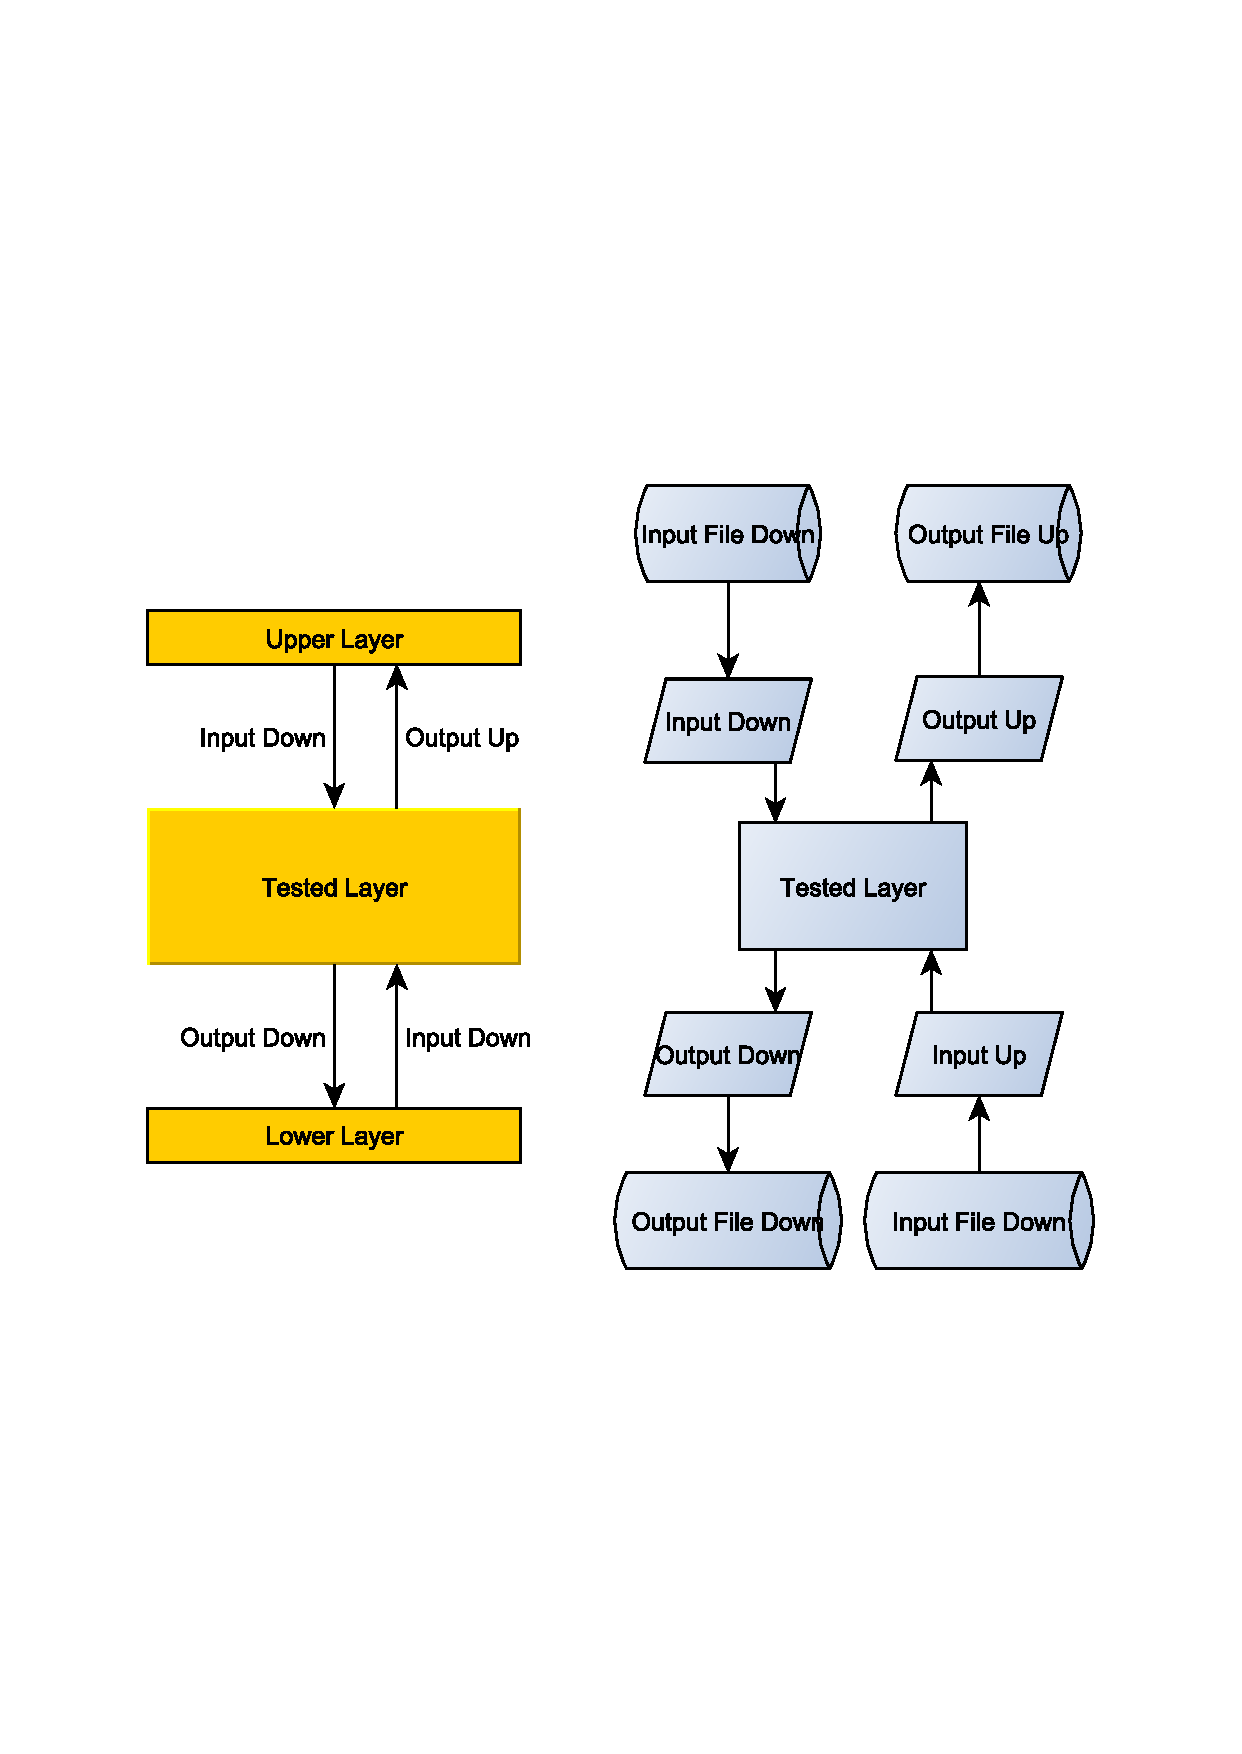
\includegraphics[scale=0.5,trim=0 0 0 0]{Layer_inputoutput.pdf}
	\caption{Substituting surrounding layers (incomplete)}
	\label{fig:Layer_inputoutput}	
	\end{center}
\end{figure}

\begin{figure}[htb]
	\begin{center}
	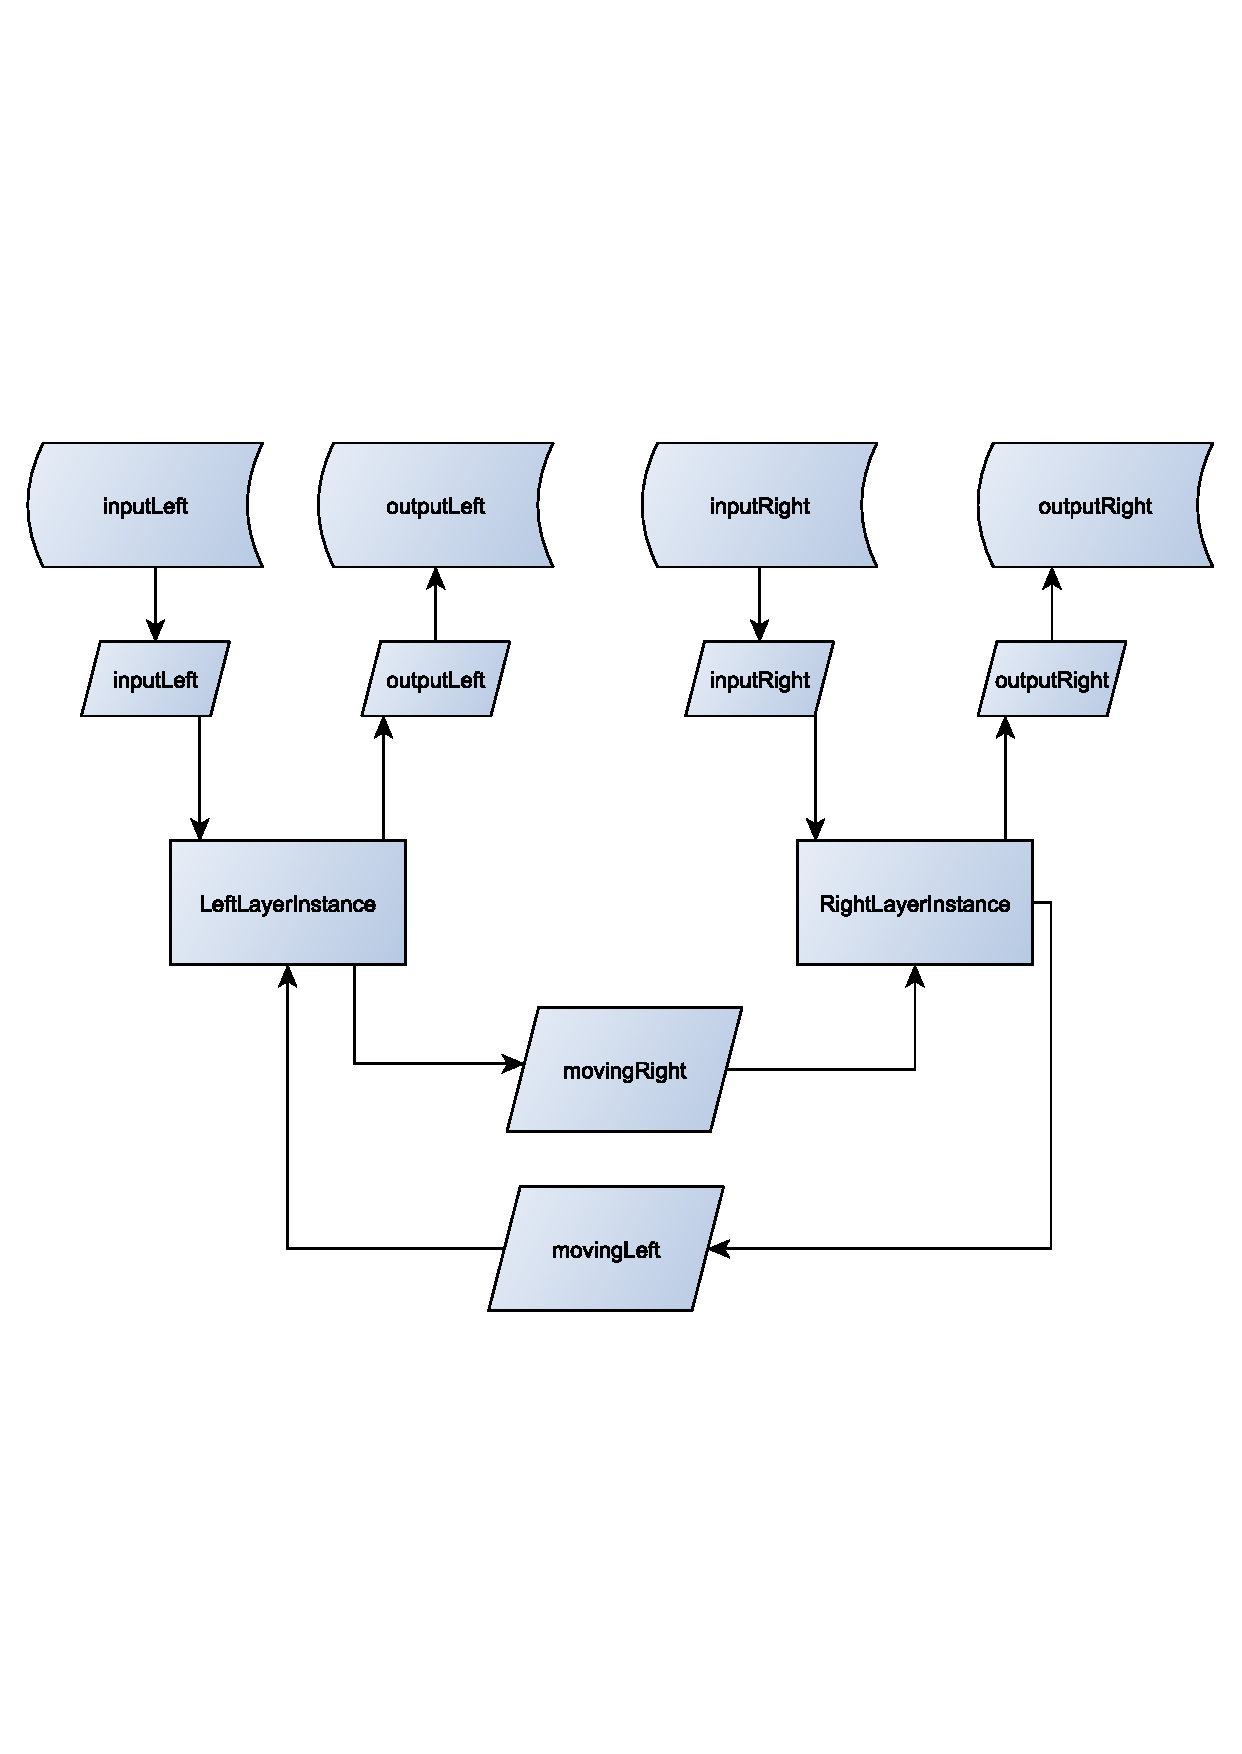
\includegraphics[scale=0.5,trim=0 0 0 0]{twoInstanceTest.pdf}
	\caption{Flowchart for test function (incomplete)}
	\label{fig:twoInstanceTest}	
	\end{center}
\end{figure}

\begin{figure}[htb]
	\begin{center}
	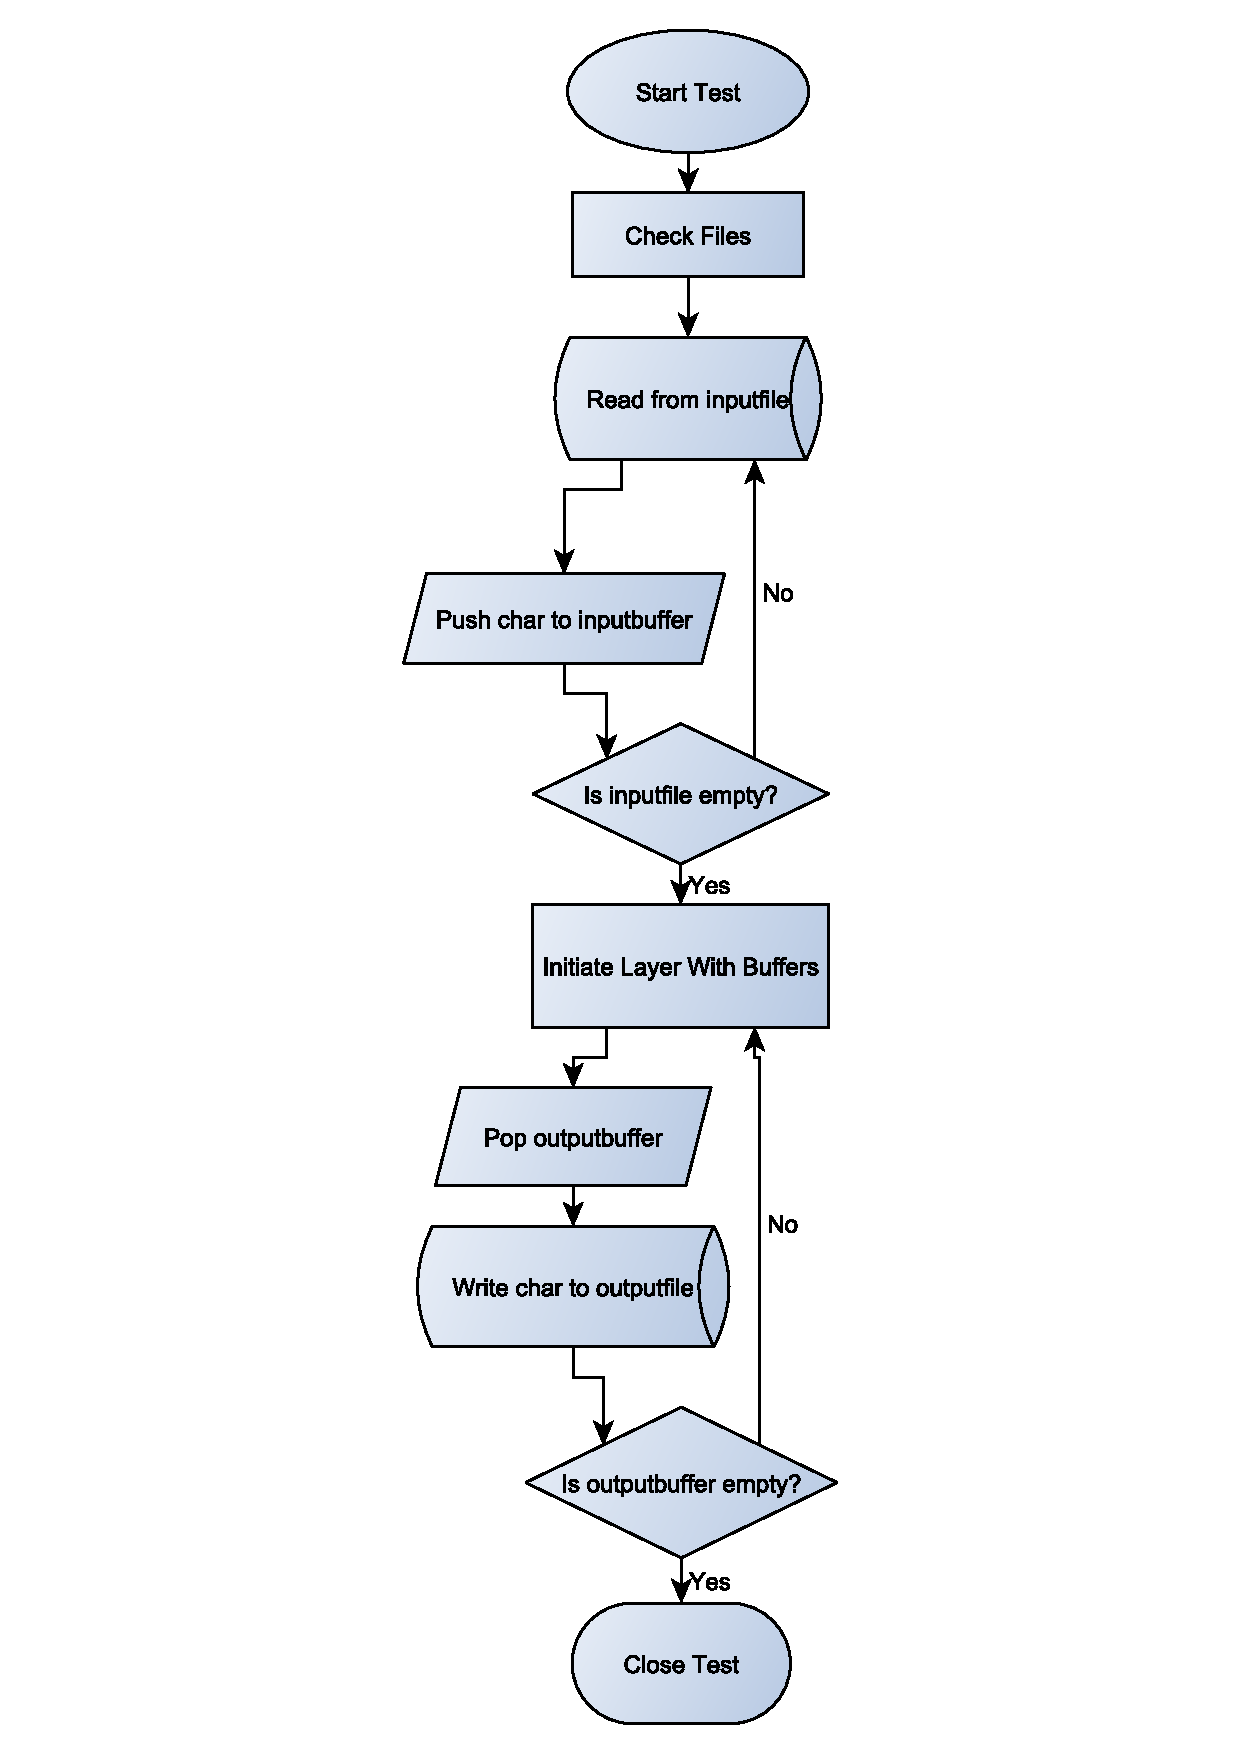
\includegraphics[scale=0.5,trim=0 0 0 0]{TestFlowchart.pdf}
	\caption{Flowchart for test function (incomplete)}
	\label{fig:TestFlowchart}	
	\end{center}
\end{figure}




\section{Test Function Documentation}
The strength in dividing development of a program into layers is that each layer can be developed and tested individually. If all layers is working individually, putting them together shouldn't be a problem. Each of the layers are therefore tested individually before the final application is created. To be able to make easy and similar tests for all the layers, it was decided that a function to make tests was developed. Though there are two different ways two test a layer, the methods are the same.

\subsection{Substituting surrounding layers}
To make it easy to change and manipulate the input and output, is it defined in .dat documents. Therefore the program doesn't have to be changed for different input, and the output can be easily extracted for further analysis. Ifstream and Ofstream are used to read and write from the documents. 
As the boost buffer is used as communication between the layers, is it also used as the test functions mean of communication with the layer tested. There are defined four buffers, two for input and two for output.
Figure \ref{fig:Layer_inputoutput}

\subsection{Testing a single instance of a layer}  

 The function is able to send data to a layer as if it was the neighbouring layers. Thus the function makes it possible to give input to a layer and check the output. This method is used to check if a layer is capable of  handling input and producing the coresponding output. This test is of course done troughout the development of the layers.


\subsection{Communication between two instances of a layer}

Another way to test a layer is to test actual communicating between two systems. In this test two instances of a layer is created, the upper layers are substituded as the single instance test. The lower layers are substituted with two buffers acting as respectivly  input and output for the two layers.The two instances can then communicate, as if the lower layers are working perfectly. This way it is possible to test if all the functions of a layer is working, when communicating with another instance of itself.
Figure \ref{fig:twoInstanceTest}


\subsection{Initiating Test}
In the beginning one simply includes the layer and in the function sets the name of the layer. It's is possible to change the defined names for the .dat files. The boost buffers are defined for the layer, so with this setup it's just running the program.
Figure \ref{fig:TestFlowchart} shows the flowchart testing a single layer by feeding input to the inputbuffer, and after initiating the layer, collecting the outbut from the outputbuffer.

\subsection{Psycical Layer}

The single instance test, wheter the computer is able to send and recieve sound have already been done while developing the layer. Therefore it is more logical to perform a test with two instances of the layer. Examening how many of the sent messages actually recieved by the other instance.

\subsection{Datalink Layer}


One of the Datalink Layers main responcebilities is keeping track of the token giving permission to send and framing the messages before they are sent.
To test that the framing are done properly, a test of a single instance of the datalink layer is tested.

 To test that a two instance test is needed, where messages and the token is sent between the to instances. 


\subsection{Transport Layer}

The transport layer is responsiple verifying the checksum. An appropriate test is sending a stream of messages to the transport layer, to see if only the correctly checksummed arrive. With the two instance test it would be possible to see if the transport layer is able produce and interpretate the checksum.

\subsection{Application Layer}

The application layer is the user of our programs interface. It is able to easily recieve data as input and forward it to the transport layer  so that it can be sent. And recieving input from the transport layer and present it properly to the user.


This is tested by creating a user program that sends files using the application layer. Transfering a file using the application layers built-in function. 

\subsection{Combined Layers}

In this test all the layers are connected and controlled by the backbone. With the file transfer program from the application layer, it is now tested by sending the file betwen two computers.